\renewcommand{\theequation}{\theenumi}
\renewcommand{\thefigure}{\theenumi}
\begin{enumerate}[label=\thesection.\arabic*.,ref=\thesection.\theenumi]
\numberwithin{equation}{enumi}
\numberwithin{figure}{enumi}
\numberwithin{table}{enumi}

\item The probability that a ticketless traveler is caught during a trip is 0.1. If the traveler makes 4 trips , the probability that he/she will be caught during at least one of the trips is:\\
\begin{enumerate}
    \item $1-(0.9)^4$
    \item $(1-0.9)^4$
    \item $1-(1-0.9)^4$
    \item $(0.9)^4$
\end{enumerate}
\solution
Let $X_i\in\cbrak{0,1}$ represent the ith trip where 1 denotes a ticketless traveller is caught.
Given,
\begin{align}
     \pr{X_i=1}&=p=0.1 \label{dec2015-3:a}
\end{align}
Let,
\begin{align}
    X=\sum_{i=1}^n X_i
\end{align}
where n is the number of trips and X has a binomial distribution.
\begin{align}
    p_X(k)&=
    \begin{cases}
     \comb{n}{k}\,p^K(1-p)^{n-k}, & 0\le k\le n
     \\
    0, & otherwise
    \end{cases}\label{dec2015-3:z}
\end{align}
As he/she makes 4 trips in total, Using \eqref{dec2015-3:a} and
\eqref{dec2015-3:z},
\begin{align}
    \pr{X=0}&=p_X(0)\\
    &=\comb{4}{0}\,p^0(1-p)^4\\
    \pr{X=0}&=(0.9)^4\label{dec2015-3:2}
\end{align}
Then probability of being caught in atleast one trip is,(Using \eqref{dec2015-3:2})
\begin{align}
    \pr{X\ge1}&=1-\pr{X<1}\\
    &=1-\pr{X=0}\label{dec2015-3:1}\\
    &=1-(0.9)^4
\end{align}

\item Suppose that $(X,Y)$ has a joint probability distribution with the marginal distribution of $X$ being N(0,1) and $E(Y|X=x)=x^3$ for all $x \in R$. Then, which of the following statements are true?
\begin{enumerate}
    \item Corr$(X,Y) = 0$
    \item Corr$(X,Y) > 0$
    \item Corr$(X,Y) < 0$
    \item X and Y are independent
\end{enumerate}
\solution
The following result shall be useful later. For $n \in N$
\begin{align}
    \int_{-\infty}^{\infty} \dfrac{x^n e^{\frac{-x^2}{2}}}{\sqrt{2\pi}}dx = 
    \begin{cases}
    0 & n\; is\; odd\\
    (n-1)\times...\times3\times1 & n\; is\; even
    \end{cases}
\end{align}
The proof for the above can be found at the end of the solution.
\begin{align}
    Corr(X,Y) = \cfrac{\sigma_{XY}^2}{\sigma_X\sigma_Y}
    \label{dec2015-108:correlationofxy}
\end{align}
We know $X \sim N(0,1)$. Thus,
\begin{align}
    f_X(x) &= \dfrac{e^{\frac{-x^2}{2}}}{\sqrt{2\pi}}\\
    E(X) &= 0\\
    \sigma_X^2 &= 1
\end{align}
\begin{align}
    \sigma_Y^2 = E(Y^2) - E(Y)^2
    \label{dec2015-108:varianceofy}
\end{align}
\begin{align}
    E(Y) &= \int_{-\infty}^{\infty}E(Y|X=x)f_X(x)dx\\
         &= \int_{-\infty}^{\infty}\dfrac{x^3 e^{\frac{-x^2}{2}}}{\sqrt{2\pi}}dx\\
         &= 0
\end{align}
\begin{align}
    E(Y^2) &= \int_{-\infty}^{\infty}E(Y^2|X=x)f_X(x)dx\\
           &= \int_{-\infty}^{\infty}\dfrac{x^6 e^{\frac{-x^2}{2}}}{\sqrt{2\pi}}dx\\
           &= 15
\end{align}
Substituting in \eqref{dec2015-108:varianceofy}
\begin{align}
    \sigma_Y^2 = 15
\end{align}
\begin{align}
    \sigma_{XY}^2 = E(XY) - E(X)E(Y)
    \label{dec2015-108:covarianceofxy}
\end{align}
\begin{align}
    E(XY) &= \int_{-\infty}^{\infty}E(XY|X=x)f_X(x)dx\\
          &= \int_{-\infty}^{\infty}E(xY|X=x)f_X(x)dx\\
          &= \int_{-\infty}^{\infty}xE(Y|X=x)f_X(x)dx\\
          &= \int_{-\infty}^{\infty}\dfrac{x^4 e^{\frac{-x^2}{2}}}{\sqrt{2\pi}}dx\\
          &= 3
\end{align}
Substituting in \eqref{dec2015-108:covarianceofxy}
\begin{align}
    \sigma_{XY}^2 = 3
\end{align}
Substituting in \eqref{dec2015-108:correlationofxy}
\begin{align}
    Corr(X,Y) = \cfrac{3}{\sqrt{15}} > 0
\end{align}
Since $Corr(X,Y) \ne 0$, X and Y are dependent. Thus option 2 is the only correct option.
\textbf{Proof for the integral:}
If n is odd, $\dfrac{x^n e^{\frac{-x^2}{2}}}{\sqrt{2\pi}}$ is an odd function, thus
\begin{align}
    \int_{-\infty}^{\infty} \dfrac{x^n e^{\frac{-x^2}{2}}}{\sqrt{2\pi}}dx = 0
\end{align}
If n is even, 
\begin{align}
    \int_{-\infty}^{\infty} \dfrac{x^n e^{\frac{-x^2}{2}}}{\sqrt{2\pi}}dx = \int_{-\infty}^{\infty} (x^{n-1}) (\dfrac{x e^{\frac{-x^2}{2}}}{\sqrt{2\pi}})dx
\end{align}
Using integration by parts,
\begin{multline}
    \int_{-\infty}^{\infty} \dfrac{x^n e^{\frac{-x^2}{2}}}{\sqrt{2\pi}}dx = \left(x^{n-1}\int \dfrac{x e^{\frac{-x^2}{2}}}{\sqrt{2\pi}}dx\right)\biggr \vert_{-\infty}^{\infty}\\
       - (n-1)\int_{-\infty}^{\infty}x^{n-2}\left(\int \dfrac{x e^{\frac{-x^2}{2}}}{\sqrt{2\pi}}dx\right) dx
\end{multline}
\begin{align}
    &= \left(x^{n-1}(-\dfrac{e^{\frac{-x^2}{2}}}{\sqrt{2\pi}})\right)\biggr \vert_{-\infty}^{\infty}
           - (n-1)\int_{-\infty}^{\infty}x^{n-2}(-\dfrac{e^{\frac{-x^2}{2}}}{\sqrt{2\pi}}) dx\\
    &= (n-1)\int_{-\infty}^{\infty} \dfrac{x^{n-2} e^{\frac{-x^2}{2}}}{\sqrt{2\pi}}dx\\
    &= (n-1)(n-3)\int_{-\infty}^{\infty} \dfrac{x^{n-4} e^{\frac{-x^2}{2}}}{\sqrt{2\pi}}dx\\
    &= (n-1)\times...\times3\times1\int_{-\infty}^{\infty} \dfrac{x^0 e^{\frac{-x^2}{2}}}{\sqrt{2\pi}}dx\\
    &= (n-1)\times...\times3\times1
\end{align}
%
 \item Let $X_1,X_2,...,X_n$ be independent and identically distributed, each having a uniform distribution on $(0,1)$. Let $S_n=\sum_{i=1}^{n}X_i$ for $n\ge 1$. Then, which of the following statements are true? 
\begin{enumerate}[label=\Alph*)]
\item $\frac{S_n}{n \log{n}}\to 0 \text{ as } n \to \infty$ with probability 1.
\item $\pr{\brak{S_n>\frac{2n}{3}}\text{occurs for infinitely many n}}=1$
\item $\frac{S_n}{\log{n}}\to 0\text{ as } n \to \infty$ with probability 1.
\item $\pr{\brak{S_n>\frac{n}{3}}\text{occurs for infinitely many n}}=1$
\end{enumerate}
%
\solution
\begin{table}[htp]
\centering
    \resizebox{\columnwidth}{20mm}{
\begin{tabular}{ |c|c|c|} 
\hline
\textbf{Symbol} & \textbf{expression/definition} \\
\hline
$S_n$ & $\displaystyle \sum_{i=1}^{n}X_i$  \\
\hline
$\mu_n$ & $\displaystyle \frac{1}{n} \sum_{i=1}^{n}X_i$  \\
\hline
& Independent continuous random\\$X$&variable identical to $X_1,X_2,...,X_n$ \\
\hline
\end{tabular}}
\caption{Variables and their definitions}
\label{dec2015-106:table1}
\end{table}
\begin{enumerate}
\item 
Given
\begin{align}
\displaystyle S_n=\sum_{i=1}^{n}X_i , n\ge 1
\end{align}
Dividing by $n$ on both sides
\begin{align}
\dfrac{S_n}{n}=\displaystyle\frac{1}{n} \sum_{i=1}^{n}X_i=\mu_n
\end{align}
It can be said that $X_1,X_2,...,X_n$ are the trials of $X$. By definition
\begin{align}
E\sbrak{X}&=\displaystyle \lim_{n\to \infty} \frac{\sum_{i=1}^{n}X_i}{n}=\lim_{n\to \infty} \frac{S_n}{n}\\
&\lim_{n\to \infty} \frac{S_n}{n}=E\sbrak{X}=\frac{1}{2} \label{dec2015-106:eq:mu_value} \\
\therefore&\lim_{n\to \infty} \frac{S_n}{n\log{n}}=0
\end{align}
\item
Using weak law, \eqref{dec2015-106:eq:mu_value}, and table \eqref{dec2015-106:table1}
\begin{align}
\lim_{n\to\infty} \pr{\abs{\mu_n-E\sbrak{X}}>\epsilon}=0, \forall \epsilon >0\\
\displaystyle \lim_{n\to\infty} \pr{S_n=\frac{n}{2}}=1 \label{dec2015-106:eq:weak_law}
\end{align}
It can be easily implied from \eqref{dec2015-106:eq:weak_law} that option B is false.
\item 
It is easy to observe from \eqref{dec2015-106:eq:mu_value} that option C is false.
\item
Using \eqref{dec2015-106:eq:weak_law}, we get
\begin{align}
\pr{\brak{S_n>\frac{n}{3}}\text{occurs for infinitely many n}}=1
\end{align}
\end{enumerate}
%
\item A fair coin is tossed repeatedly. Let $X$ be the number of tails before the first heads occurs. Let $Y$ denote the number of tails between the first and second heads. Let $X+Y = N$. Then which of the following are true?
\begin{enumerate}
    \item X and Y are independent random variables with
    {\footnotesize
    \begin{align}
        \pr{X = k} = \pr{Y = k} =
        \begin{cases}
            2^{-(k+1)} & k=0,1,2 \ldots
            \\
            0 & otherwise
        \end{cases}
    \end{align}
    }
    \item $N$ has a probability mass function given by
    {\small
     \begin{align}
        \pr{N = k} =
        \begin{cases}
            (k-1)2^{-k} & k=2,3,4 \ldots
            \\
            0 & otherwise
        \end{cases}
    \end{align}
    }
    \item Given $N = n$, the conditional distribution of X and Y are independent
    \item Given $N = n$
     \begin{align}
        \pr{X = k} =
        \begin{cases}
            \frac{1}{n+1} & n=0,1,2 \ldots
            \\
            0 & otherwise
        \end{cases}
    \end{align}
\end{enumerate}
%
\item An urn has 3 red and 6 black balls. Balls are drawn at random one by one without replacement. The probability that second red ball appears on fifth draw is: \\
\begin{enumerate}
    \item $\frac{1}{9!}$
    \newline
    \item $\frac{4!}{9!}$
    \newline
    \item $4\brak{\frac{6!4!}{9!}}$
    \newline
    \item $\frac{6!4!}{9!}$
\end{enumerate}
%
%
\solution
 To obtain a second red ball at the fifth draw, the first 4 trials should involve drawing only 1 red ball out of the 3 and 3 black balls out of the 6. Probability of this happening:
 \begin{align}
  \frac{\comb{3}{1}\comb{6}{3}}{\comb{9}{4}}
     \end{align}
The probability of the fifth ball turning out to be red is:
\begin{align}
    \frac{\comb{2}{1}}{\comb{5}{1}}
\end{align}
By Multiplication rule, total probability:
\begin{align}
    \frac{\comb{3}{1}\comb{6}{3}\comb{2}{1}}{\comb{5}{1}\comb{9}{4}}
    = \frac{3!\times 6!\times2!\times4!\times4!\times5!}{2!\times3!\times3!\times5!\times9!}\\ 
    =4\brak{\frac{4!6!}{9!}}
\end{align}

%
\item Let $X_i 's$ be independent random variables such that $X_i 's$ are symmetric about 0 and $var(X_i)=2i - 1$,for $i\geq 1$.then,
$\lim_{n \to \infty}\pr{X_1 +X_2 + \dots + X_n > n\log{n}}$
\begin{enumerate}
\begin{multicols}{2}
\setlength\itemsep{2em}
\item does not exist.
\item equals $\dfrac{1}{2}$.\\
\item equals 1.
\item equals 0.
\end{multicols}
\end{enumerate}
%
\solution
Let $X= X_1 +X_2 + \dots + X_n $,
as $X_i 's$ are symmetric about 0.
The mean of X is given by,
\begin{align}
E[X]=0 \label{dec2015-53:a}
\end{align}
the variance of X is given by,
\begin{align}
var[X]&= \sum_{i=1}^{n}(2i -1)\\
   &= \frac{2n(n+1)}{2} - n\\
   &= n^{2}
\end{align}
the standard deviation,
\begin{align}
\sigma_X = n \label{dec2015-53:b}
\end{align}
Applying Chebyshev's Inequality for the random variable X, for any $k>0$
\begin{align}
\pr{\abs{X-E[X]}> k\sigma_X} \leq \frac{1}{k^{2}} \label{dec2015-53:c}
\end{align}
let $k=\log{n} $ ,
using \eqref{dec2015-53:a} and \eqref{dec2015-53:b} in \eqref{dec2015-53:c},
\begin{align}
\pr{\abs{X}> n\log{n}} \leq \frac{1}{(\log{n})^{2}}\\
\pr{X> n\log{n}} + \pr{X< -n\log{n}} \leq \frac{1}{(\log{n})^{2}} \label{dec2015-53:e}
\end{align}
As, X is symmetric about 0,
\begin{align}
\pr{X> n\log{n}} =\pr{X< -n\log{n}} \label{dec2015-53:f}
\end{align}
using \eqref{dec2015-53:f} in \eqref{dec2015-53:e},
\begin{align}
2\pr{X> n\log{n}} \leq \frac{1}{(\log{n})^{2}}\\
\pr{X> n\log{n}} \leq \frac{1}{2(\log{n})^{2}}
\end{align}
as any probability is greater than 0,
\begin{align}
0< \pr{X> n\log{n}} \leq \frac{1}{2(\log{n})^{2}} \label{dec2015-53:d}
\end{align}
applying sandwich principle to \eqref{dec2015-53:d},
\begin{align}
\lim_{n \to \infty} 0< \lim_{n \to \infty} \pr{X> n\log{n}} \leq \lim_{n \to \infty} \frac{1}{2(\log{n})^{2}}\\
\lim_{n \to \infty}\pr{X_1 +X_2 + \dots + X_n > n\log{n}} = 0
\end{align}
Hence the option.4 is correct.
%
\item Suppose
$\begin{pmatrix}
X\\
Y
\end{pmatrix}$ is a random vector such that the marginal distribution of $X$ and the marginal distribution of $Y$ are the same and each is normally distributed with mean 0 and variance 1. Then, which of the following conditions imply independence of $X$ and $Y?$
\begin{enumerate}
\item Cov$\brak{X,Y}=0$
\item $aX+bY$ is normally distributed with mean 0 and variance $a^2+b^2$ for all real $a$ and $b$
\item $\pr{X\le 0, Y\le0}=\frac{1}{4}$
\item $E\sbrak{e^{itX+isY}}=E\sbrak{e^{itX}}E\sbrak{e^{isY}}$ for all real $s$ and $t$
\end{enumerate}
%
\solution


An important property of dirac delta function that will be used at multiple ocassions in this solution is
\begin{align}
\displaystyle\int\limits_{-\infty}^{\infty} f(x)\delta(x-a)dx=f(a) \label{dec/2015/109/eq:dirac}
\end{align}
Given $X\sim N\brak{0,1}, Y\sim N(0,1)$
\begin{enumerate}
\item
\begin{align}
Cov(X,Y)=0\\
E\sbrak{XY}-E\sbrak{X}E\sbrak{Y}=0\\
E\sbrak{XY}=0\\
\displaystyle \int\limits_{-\infty}^{\infty} \int\limits_{-\infty}^{\infty}xyf_{XY}(x,y) dxdy=0
\end{align}
This doesn't imply independence. Counter example given below\\
Lets consider a case where $X$ and $Y$ are dependent based on the following relation, $Y$ being independent of $K$
\begin{align}
X=KY \label{dec/2015/109/eq:case}
\end{align}
PMF for $K$ is given as
\begin{align}
p_K(k)=
\begin{cases}
\frac{1}{2} &k=1\\
\frac{1}{2} & k=-1\\
0 & \text{otherwise}
\end{cases}
\end{align}
A simulation is given below, Y is gaussian, then X also follows gaussian
\begin{figure}[!ht]
\centering
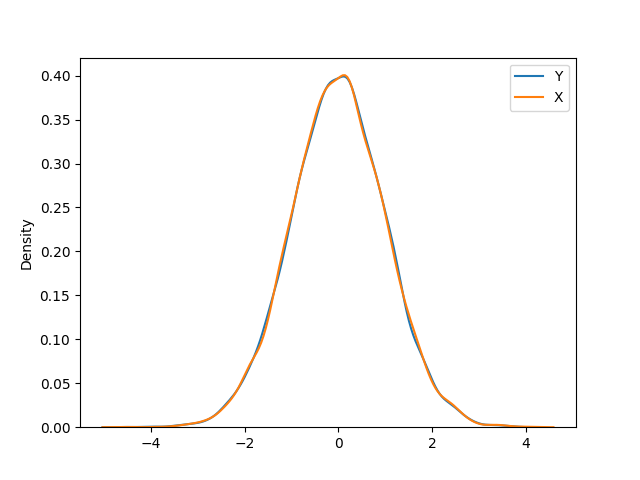
\includegraphics[width=\columnwidth]{solutions/2015/dec/109/figure/fig.png}
\caption{X and Y, if Y is normal}
\label{fig:dec/2015/109/plot}
\end{figure}
Theoretically it can be proved in the following manner,
Since $K$ and $Y$ are independent
\begin{align}
f_X(x)&=\pr{K=1}f_Y(x)+\pr{K=-1}f_Y(-x)\\
&=\frac{1}{2}\brak{f_Y(x)+f_Y(-x)}\\
&=f_Y(x)
\end{align}
Therefore, $X$ follows identical but not independent distribution as $Y$, An alternative proof is given below as a proof for marginal probability\\
Now consider that $X$ is normally distributed, we will establish $Y$ is also normally distributed.
The joint probability distribution is therefore
\begin{align}
f_{XY}(x,y)&=f_{X|Y}(x|y)f_X(x)\nonumber \\
&=f_X(x)\frac{1}{2}(\delta(x+y)+\delta(x-y))\label{dec/2015/109/eq:counter}
\end{align}
The marginal probability distribution function for $X$ is given as
\begin{align}
\int\limits_{-\infty}^{\infty}f_X(x)\frac{1}{2}(\delta(x+y)+\delta(x-y)) dy
\end{align}
Using \eqref{dec/2015/109/eq:dirac}, we get
\begin{align}
\int\limits_{-\infty}^{\infty}f_X(x)\frac{1}{2}(\delta(x+y)+\delta(x-y))dy=f_X(x)
\end{align}
We know that $X\sim N(0,1)$, $f_X(x)$ represents gaussian probability distribution function.\\
Futher, using symmetry of \eqref{dec/2015/109/eq:case}, we can establish that marginal distribution of $Y$ is gaussian. Here is a proof anyways
\begin{align}
f_Y(y)=\int\limits_{-\infty}^{\infty}f_X(x)\frac{1}{2}(\delta(x+y)+\delta(x-y)) dx
\end{align}
Using \eqref{dec/2015/109/eq:dirac}, we get
\begin{align}
f_Y(y)=\frac{1}{2}\brak{f_X(y)+f_X(-y)}=f_X(y)
\end{align}
Since $Y$ has identical probability distribution function, $Y\sim N(0,1)$\\
The covariance is given as
\begin{align}
&Cov(X,Y)=E[XY]-E[X]E[Y]=E[XY]\\
&E[XY]=\int\limits_{-\infty}^{\infty}\int\limits_{-\infty}^{\infty}xyf_{XY}(x,y) dy dx
\end{align}
\begin{align}
=\int\limits_{-\infty}^{\infty}\int\limits_{-\infty}^{\infty}xyf_X(x)\frac{1}{2}(\delta(x+y)+\delta(x-y)) dy dx\\
=\int\limits_{-\infty}^{\infty} xf_X(x)\int\limits_{-\infty}^{\infty}y\frac{1}{2}(\delta(x+y)+\delta(x-y)) dy dx
\end{align}
Using \eqref{dec/2015/109/eq:dirac}
\begin{align}
E[XY]=\int\limits_{-\infty}^{\infty}xf_X(x)\frac{1}{2}(x-x)dx=0
\end{align}
\item
Defining the following matrices/vectors
\begin{table}[h!]
\centering
\begin{tabular}{ |c|c|} 
\hline
\textbf{vector/matrix} & \textbf{expression} \\
\hline&\\[-1em]
$\boldsymbol{Z}$& $\begin{pmatrix} X &Y\end{pmatrix}^\top$\\[2pt]
\hline&\\[-1em]
$\boldsymbol{C}$&$\begin{pmatrix} a &b\end{pmatrix}^\top$  \\[2pt]
\hline&\\[-1em]
$\boldsymbol{\mu}$&$\begin{pmatrix} 0 &0\end{pmatrix}^\top$  \\[2pt]
\hline&\\[-1em]
$\boldsymbol{\Sigma}$&$\begin{pmatrix}1&\rho\\\rho&1\end{pmatrix}$ \\
\hline
\end{tabular}
\caption{vectors/matrices and their expressions}
\label{dec/2015/109/table1}
\end{table}
Given
\begin{align}
\boldsymbol{C^\top Z}\sim N\brak{0,a^2+b^2}
\end{align}
Since this is true for all $a$ and $b$, it is equivalent to $X$ and $Y$ being jointly gaussian
\begin{align}
\boldsymbol{Z}\sim N(\boldsymbol{\mu},\boldsymbol{\Sigma})
\end{align}
For correlated random variables $X$ and $Y$ in bivariate normal distribution, we have
\begin{align}
\sigma_{Z}^2=\displaystyle\sum_{i,j}\Sigma_{ij}\\
a^2+b^2=a^2+b^2+2\rho ab\\
\therefore \rho=0\label{dec/2015/109/eq:rho}
\end{align}
The joint distribution is given as
\begin{align}
f_{\boldsymbol{Z}}(x,y)=\frac{\text{exp}\brak{-\frac{1}{2}\brak{\boldsymbol{z-\mu}}^\top\boldsymbol{\Sigma}^{-1}\brak{\boldsymbol{z-\mu}}}}{\sqrt{(2\pi)^2\abs{\boldsymbol{\Sigma}}}}\\
f_{\boldsymbol{Z}}(x,y)=\frac{\text{exp}\brak{-\frac{1}{2}{\begin{pmatrix} x &y\end{pmatrix}} I_2{\begin{pmatrix} x &y\end{pmatrix}}^\top}}{\sqrt{(2\pi)^2}}
\end{align}
Where $I_2$ is the identity matrix of order 2
\begin{align}
f_{\boldsymbol{Z}}(x,y)=\frac{\text{exp}\brak{-\frac{1}{2}{\begin{pmatrix} x &y\end{pmatrix}} {\begin{pmatrix} x &y\end{pmatrix}}^\top}}{\sqrt{(2\pi)^2}}\\
f_{\boldsymbol{Z}}(x,y)=\frac{\text{exp}\brak{-\frac{1}{2}\brak{x^2+y^2}}}{\sqrt{(2\pi)^2}}=f_X(x)f_Y(y)
\end{align}
$\therefore$ \textbf{Option(2) is correct}, A simulation for bivariate gaussian is given below
\begin{figure}[!ht]
\centering
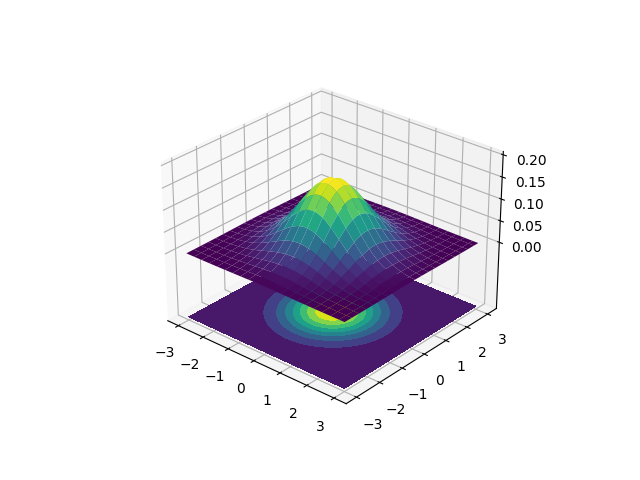
\includegraphics[width=\columnwidth]{solutions/2015/dec/109/figure/plot.png}
\caption{bivariate gaussian while 0 mean vector and identity covariance matrix}
\label{dec/2015/109/plot}
\end{figure}
\item
\begin{align}
\pr{X\le 0, Y\le0}=\frac{1}{4}
\end{align}
This doesn't imply independence, it can be true even for dependent $X$ and $Y$, the counter example is \eqref{dec/2015/109/eq:counter}, the joint probability function is symmetric across all 4 quadrants
\begin{align}
\therefore \pr{X\le 0, Y\le0}=\frac{1}{4}
\end{align}
Alternatively, here is proof 
\begin{align}
\pr{X\le 0}=F_X(0)=\frac{1}{2} \label{dec/2015/109/eq:pr1}
\end{align}
Using \eqref{dec/2015/109/eq:case}
\begin{align}
\pr{Y\le 0|X\le 0}=\frac{1}{2} \label{dec/2015/109/eq:pr2}
\end{align}
Using \eqref{dec/2015/109/eq:pr1} and \eqref{dec/2015/109/eq:pr2}
\begin{align}
\pr{X\le 0, Y\le0}=\frac{1}{4}
\end{align}
\item
\begin{align}
E\sbrak{e^{itX+isY}}=E\sbrak{e^{itX}}E\sbrak{e^{isY}}\\
E\sbrak{e^{itX+isY}}=\varphi_X(t)\varphi_Y(s) \label{dec/2015/109/eq:inde}
\end{align}
The inverse is given as
\begin{align}
f_{XY}(x,y)=\frac{1}{4\pi^2}\displaystyle \int\limits_{-\infty}^{\infty} \int\limits_{-\infty}^{\infty} e^{-itX-isY}E\sbrak{e^{itX+isY}}ds dt
\end{align}
Using \eqref{dec/2015/109/eq:inde}
\begin{align}
f_{XY}(x,y)&=\frac{1}{4\pi^2}\displaystyle \int\limits_{-\infty}^{\infty} \int\limits_{-\infty}^{\infty} e^{-itX-isY}\varphi_X(t)\varphi_Y(s) ds dt\\
&f_{XY}(x,y)=f_X(x)f_Y(y)
\end{align}
$\therefore$ \textbf{Option(4) is correct}
\end{enumerate}




\end{enumerate}
